\documentclass[11pt,a4paper]{article}
\usepackage[margin=2.3cm]{geometry}
\usepackage{amsmath,amssymb}
\usepackage{graphicx}
\usepackage{booktabs}
\usepackage{xcolor}
\usepackage[font=small,labelfont=bf]{caption}
\usepackage{microtype}
\usepackage{placeins}
\usepackage{rotating}
\usepackage{braket}
\usepackage[skins,breakable]{tcolorbox}
\usepackage[colorlinks=true,linkcolor=blue!50!black,citecolor=blue!50!black,urlcolor=blue!50!black]{hyperref}
\usepackage[capitalise,nameinlink]{cleveref}  % load after hyperref
\graphicspath{{../rydberg/figs/}}
\emergencystretch=3em

\newtcolorbox{finding}[1][]{enhanced,breakable,colback=blue!4,colframe=blue!50!black,
  fonttitle=\bfseries,title={Finding#1}}
\newtcolorbox{definition}[1][]{enhanced,breakable,colback=black!3,colframe=black!45,
  fonttitle=\bfseries,title={Definition#1}}

% one colour per family, the same hex values as B2B_COLORS in rydberg_figs.py
\definecolor{cBW}{HTML}{000000}   % Baxter-Wu
\definecolor{cNM}{HTML}{FF0000}   % Newman-Moore
\definecolor{cTC}{HTML}{0000FF}   % toric code, diagonal field
\definecolor{cXM}{HTML}{CC79A7}   % Xu-Moore
\definecolor{cRy}{HTML}{56B4E9}   % Rydberg Ising reference
\newcommand{\BW}{\textcolor{cBW}{\textbf{Baxter--Wu quench}}}
\newcommand{\NM}{\textcolor{cNM}{\textbf{Newman--Moore quench}}}
\newcommand{\TC}{\textcolor{cTC}{\textbf{toric-code quench}}}
\newcommand{\XM}{\textcolor{cXM}{\textbf{Xu--Moore quench}}}

\newcommand{\tmu}{t^*_\mu}
\newcommand{\tw}{t^*_w}
\newcommand{\whi}{w_{hi}}
\newcommand{\Spage}{S_{\mathrm{Page}}}

\title{Multi-spin quenches: where is an RBM predicted easy and an MPS hard?}
\author{Exact-diagonalisation screen (RBM runs to follow)}
\date{30 October 2026}

\begin{document}
\maketitle

\begin{abstract}
Are there quenches with three- and four-spin interactions in which a restricted Boltzmann machine (RBM) is predicted
to follow the exact state while a matrix product state (MPS) would need a large bond dimension? We evolved seven
families on 12--18 spins exactly and computed four RBM predictors (few-body error rate $R_2$, its integral, high-order
cluster weight $\whi$, cumulant level $\mu$) and the entanglement entropy $S$. The predictors disagree. $\mu$ predicts
an easy RBM at MPS-hard times for the toric code in a diagonal field ($16$--$24\%$ of the save times for $h_f\le0.4$, 18
spins) and for the Baxter--Wu and Newman--Moore quenches at weak field ($19\%$ and $31\%$ at $h=0.05$, below $5\%$ for
$h\ge0.2$); $\whi$ calls all of these hard within $0.3$ time units. All other product-state quenches are hard by every
predictor. On two reference quenches with RBM data, $\mu$ tracks the infidelity best (Spearman $0.91$, $0.93$) but can
be late by up to $2.6\times$. RBM runs are needed to decide.
\end{abstract}

\begin{figure}[!b]
  \centering
  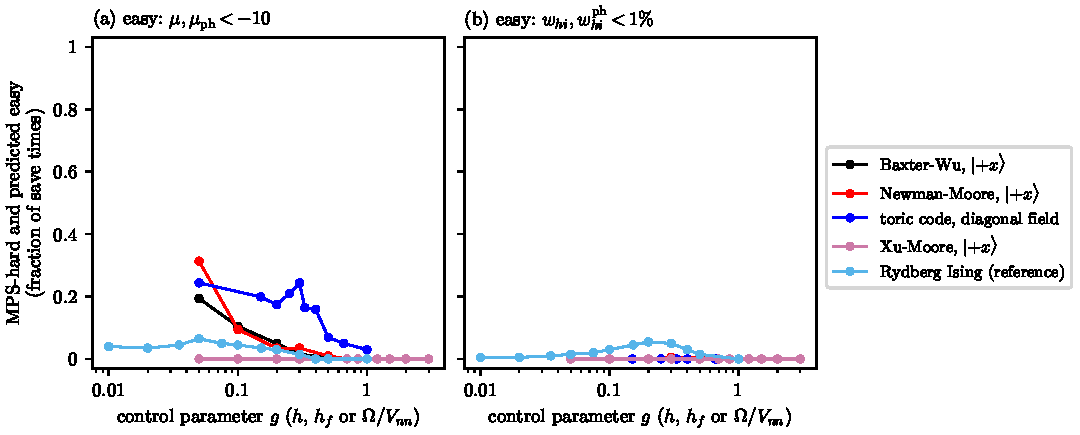
\includegraphics[width=0.7\linewidth]{b2b/windows.pdf}
  \caption{\textbf{Graphical abstract.} Fraction of the save times at which the exact state is MPS-hard (entanglement
    entropy $S\ge\Spage/2$, half the value of a random state) \emph{and} still predicted easy for an RBM, against the
    control parameter $g$ of each family (transverse field $h$, final field $h_f$, or drive $\Omega/V_{nn}$; log scale).
    (a)~``Easy'' means before both cumulant levels first exceed the threshold, $\mu,\mu_{\mathrm{ph}}<-10$.
    (b)~``Easy'' means before both high-order weights first exceed $1\%$, $\whi,\whi^{\mathrm{ph}}<0.01$.
    Families: Baxter--Wu ($-\sum_\triangle ZZZ-h\sum X$, 18 spins) and Newman--Moore ($-\sum_{\triangle_\uparrow}ZZZ-h\sum X$,
    16 spins) from $\ket{+x}$; toric code $-\sum_sA_s-\sum_pB_p-h_f\sum(Z+X)/\sqrt2$ from its ground state at $h_f=0.1$
    (18 spins); Xu--Moore ($-\sum_\square ZZZZ-h\sum X$, 16 spins) from $\ket{+x}$; the two-spin Rydberg Ising quench of the
    previous report as reference (12 spins). Not shown: the no-quench point $h_f=0.1$ and the points at $g=0$ (log
    axis; see text), the mixed families and the ground-state starts of the plaquette and triangle models
    (\cref{sec:negative}). Run lengths: $t_{\max}=\min(300,\max(10,3/h))$ for the $\ket{+x}$ starts, $10$ for the toric code.}
  \label{fig:abstract}
\end{figure}

\section{Overview}
\paragraph{Question.} The previous report on two-spin quenches found an RBM advantage over MPS only in near-classical
quenches, and argued that three- and four-spin terms freeze an RBM that starts from a product state. Are there
multi-spin quench families, with a control parameter, in which some quenches are predicted easy for an RBM while the
state is MPS-hard, and others hard?

\paragraph{Method} (\cref{sec:defs,sec:setup}). Exact evolution of 7 families (B1--B7, \cref{tab:families}) and 4
reference families on 12--18 spins, 12 values of the control parameter per family (8--13 for the references), 186 runs
in total. From the exact state $\psi(s,t)$ we compute the predictors of \cref{sec:defs} at 201 times per run. No RBM
was run in this study.

\paragraph{Answer} (\cref{sec:toric,sec:threespin,sec:negative,sec:verdict}).
\begin{itemize}
  \item \emph{Predicted easy at MPS-hard times, by $\mu$ only:} the \TC{} for $h_f\le0.4$ (\cref{sec:toric}), and the
    \BW{} and \NM{} at weak field, with windows that shrink steadily as $h$ grows (\cref{sec:threespin}).
  \item \emph{The predictors disagree on exactly these cases.} The high-order weight $\whi$ crosses $1\%$ within
    $t\approx0.3$, and $R_2$ stays between $4.9$ and $6$ in the Baxter--Wu quench.
  \item \emph{Hard by every predictor:} from $\ket{+x}$, Xu--Moore and the two mixed families, within $t\le0.6$
    (\cref{sec:negative}). Of the ground-state starts of the plaquette and triangle models, only Newman--Moore opens
    small $\mu$-windows.
  \item \emph{Two rows give no usable prediction:} the toric code in a $Z$ field (B1) stays in a sector of 256 of
    $2^{18}$ configurations, so all predictors computed in the $Z$ basis are meaningless; and the ground-state start
    of Baxter--Wu turned out to be an ordered cat state (\cref{app:issues}).
\end{itemize}

\section{Predictors}
\label{sec:defs}
All quantities refer to $N$ spins in the $Z$ basis, $s\in\lbrace\pm1\rbrace^N$, and the cluster functions
$s_A=\prod_{i\in A}s_i$ for a set $A$ of sites ($\lvert A\rvert$ is the order of the cluster). Energies are in units
of the multi-spin coupling ($J=1$), times in units of $1/J$.

\begin{definition}[: few-body error rate $R_k$ and its integral $\Phi_k$]
Write the exact evolution as $\partial_t\log\psi(s)=v(s)$ with the local velocity $v(s)=-i\,(H\psi)(s)/\psi(s)$.
The few-body error rate is the part of $v$ that no $k$-body function can match, measured with the Born weight
$p(s)=\lvert\psi(s)\rvert^2$:
\[
  R_k^2=\min_{c}\sum_s p(s)\,\Big\lvert v(s)-\sum_{\lvert A\rvert\le k}c_As_A\Big\rvert^2 ,
\]
with complex $c_A$ for all clusters up to $k$ sites (all-to-all). $R_2=0$ means that a two-body Jastrow factor can
follow the evolution exactly for an instant. The accumulated error is $\Phi_k(t)=\int_0^tR_k\,dt'$. Implementation and
checks: \cref{app:rk}.
\end{definition}

$R_2$ is the main variant. It was validated only on the transverse-field Ising chain, where an RBM represents two-body
phases exactly. For multi-spin $H$ it measures the distance to a two-body motion, which is stricter than what an RBM
with weights of order one can do; $R_4$ (clusters up to 4 sites) is shown in the appendix. $R_2$ and $\Phi_2$ have
no threshold here, because the size rescaling of the published threshold could not be checked; they are read only
as ``small'' or ``large''.

\begin{definition}[: cluster predictors $\mu$ and $\whi$]
\begin{itemize}
  \item $c_A=2^{-N}\sum_ss_A\log\lvert\psi(s)\rvert$: cluster coefficients of the log-amplitude. Coefficients with
    $\ln\lvert c_A\rvert<-28$ count as numerical noise and are dropped.
  \item \emph{Cumulant level} $\mu$: rank the remaining $N_{\mathrm{real}}$ coefficients by size and fit the rank as
    a function of $x=\ln\lvert c_A\rvert$ with the Fermi--Dirac form $N_{\mathrm{real}}/(e^{(x-\mu)/T}+1)$. So $\mu$
    is a natural logarithm, and about half of the coefficients are larger than $e^{\mu}$: $\mu=-10$ means that the
    typical relevant cluster has $\lvert c_A\rvert\approx e^{-10}\approx5\times10^{-5}$. Small $\mu$ means few
    relevant clusters. If no cluster beyond two sites survives the noise cut, $\mu=-\infty$ (shown at $-30$).
    $\mu_{\mathrm{ph}}$ is the same for the phase $\arg\psi$, unwrapped in time, with its mean removed.
  \item \emph{High-order weight} $\whi=\sum_{\lvert A\rvert>4}c_A^2/\sum_{\lvert A\rvert\ge1}c_A^2$, and
    $\whi^{\mathrm{ph}}$ for the phase. We set $\whi=0$ when the denominator is below $10^{-20}$ (flat amplitude, e.g.\
    a product state; without this the ratio of two round-off numbers exceeds $1\%$).
\end{itemize}
$\mu$ measures the \emph{absolute} size of the many-body clusters, $\whi$ their weight \emph{relative} to all clusters.
\end{definition}

\paragraph{Entanglement.} $S$: von Neumann entropy (nats) of the exact state between the first $N/2$ sites and the
rest. On the square and triangular tori the halves are two blocks of columns; on the toric-code tori they are the links
with midpoint $x\le1$ against the rest, so the cut is spatial (\cref{app:lattices}). \emph{MPS-hard} means
$S\ge\Spage/2=\tfrac12(\tfrac N2\ln2-\tfrac12)$: $1.83$, $2.52$ and $2.87$ nats for $N=12$, $16$, $18$.

\begin{definition}[: onset times and the predicted window]
\begin{itemize}
  \item $\tmu$: first time with $\mu>-10$ or $\mu_{\mathrm{ph}}>-10$.
  \item $\tw$: first time with $\whi>1\%$ or $\whi^{\mathrm{ph}}>1\%$.
  \item $t_S$: first time at which the state is MPS-hard.
  \item \emph{Predicted window} of a criterion: the fraction of the 201 save times at which the state is MPS-hard
    \emph{and} $t<t^*$ ($t^*=\tmu$ or $\tw$); $0$ if the state is never MPS-hard. At weak fields $S$ oscillates
    around the threshold, so this is smaller than the time between $t_S$ and $t^*$.
\end{itemize}
\end{definition}

The non-classicality $\eta=\lVert H-\mathrm{diag}H\rVert_F/\lVert H-\mathrm{tr}H/2^N\rVert_F$ is $0$ for a diagonal
(Ising) Hamiltonian and $1$ for a purely off-diagonal one.

\section{Setup of the highlighted quenches}
\label{sec:setup}
The main text discusses three cases; \cref{tab:families} lists all families.
\begin{itemize}
  \item \TC{} (B2): $H=-\sum_sA_s-\sum_pB_p-h_f\sum_i(Z_i+X_i)/\sqrt2$, with star $A_s=\prod_{i\in s}X_i$ and plaquette
    $B_p=\prod_{i\in p}Z_i$, on the links of a $3\times3$ torus (18 spins; also $2\times3$, 12 spins), from the ground
    state at $h_f=0.1$ (gap $1.2\times10^{-3}$). The diagonal field makes neither $A_s$ nor $B_p$ conserved. We know of
    no duality that maps this case to a two-spin model; the $Z$-field case maps to the transverse-field Ising
    model~\cite{Wegner71,Trebst07}. $\eta=0.71$.
  \item \BW{} (B4): $H=-\sum_\triangle Z_iZ_jZ_k-h\sum_iX_i$ on all triangles of an $18$-site triangular torus
    ($6\times3$, compatible with the three-sublattice order of the model~\cite{BaxterWu73}), from $\ket{+x}$, $\eta=0.04$--$0.91$.
    The \NM{} (B5)~\cite{NewmanMoore99}, with up-triangles only, on a $4\times4$ torus, behaves similarly and is
    quoted alongside.
  \item \XM{} (B3): $H=-\sum_\square Z_iZ_jZ_kZ_l-h\sum_iX_i$ on a $4\times4$ torus~\cite{XuMoore04}, from $\ket{+x}$.
    It stands for the families that are hard everywhere.
\end{itemize}
The final field $h_f$ is the control parameter of the toric code ($0$--$1$; $t_{\max}=10$), and the field $h$ that of
the $\ket{+x}$ starts ($0.05$--$3$; run length $t_{\max}=\min(300,\max(10,3/h))$).\footnote{Exact evolution
with Krylov exponentials (\texttt{expm\_multiply}) in steps of at most $\min(\Delta t_{\mathrm{save}},0.1/\lVert
H_{\mathrm{off}}\rVert_{\infty})$, $201$ save times per run. The phase is unwrapped exactly for the diagonal part and by
step-to-step continuity for the rest. Cost and data: \cref{app:numerics}.}

\begin{sidewaysfigure}
  \centering
  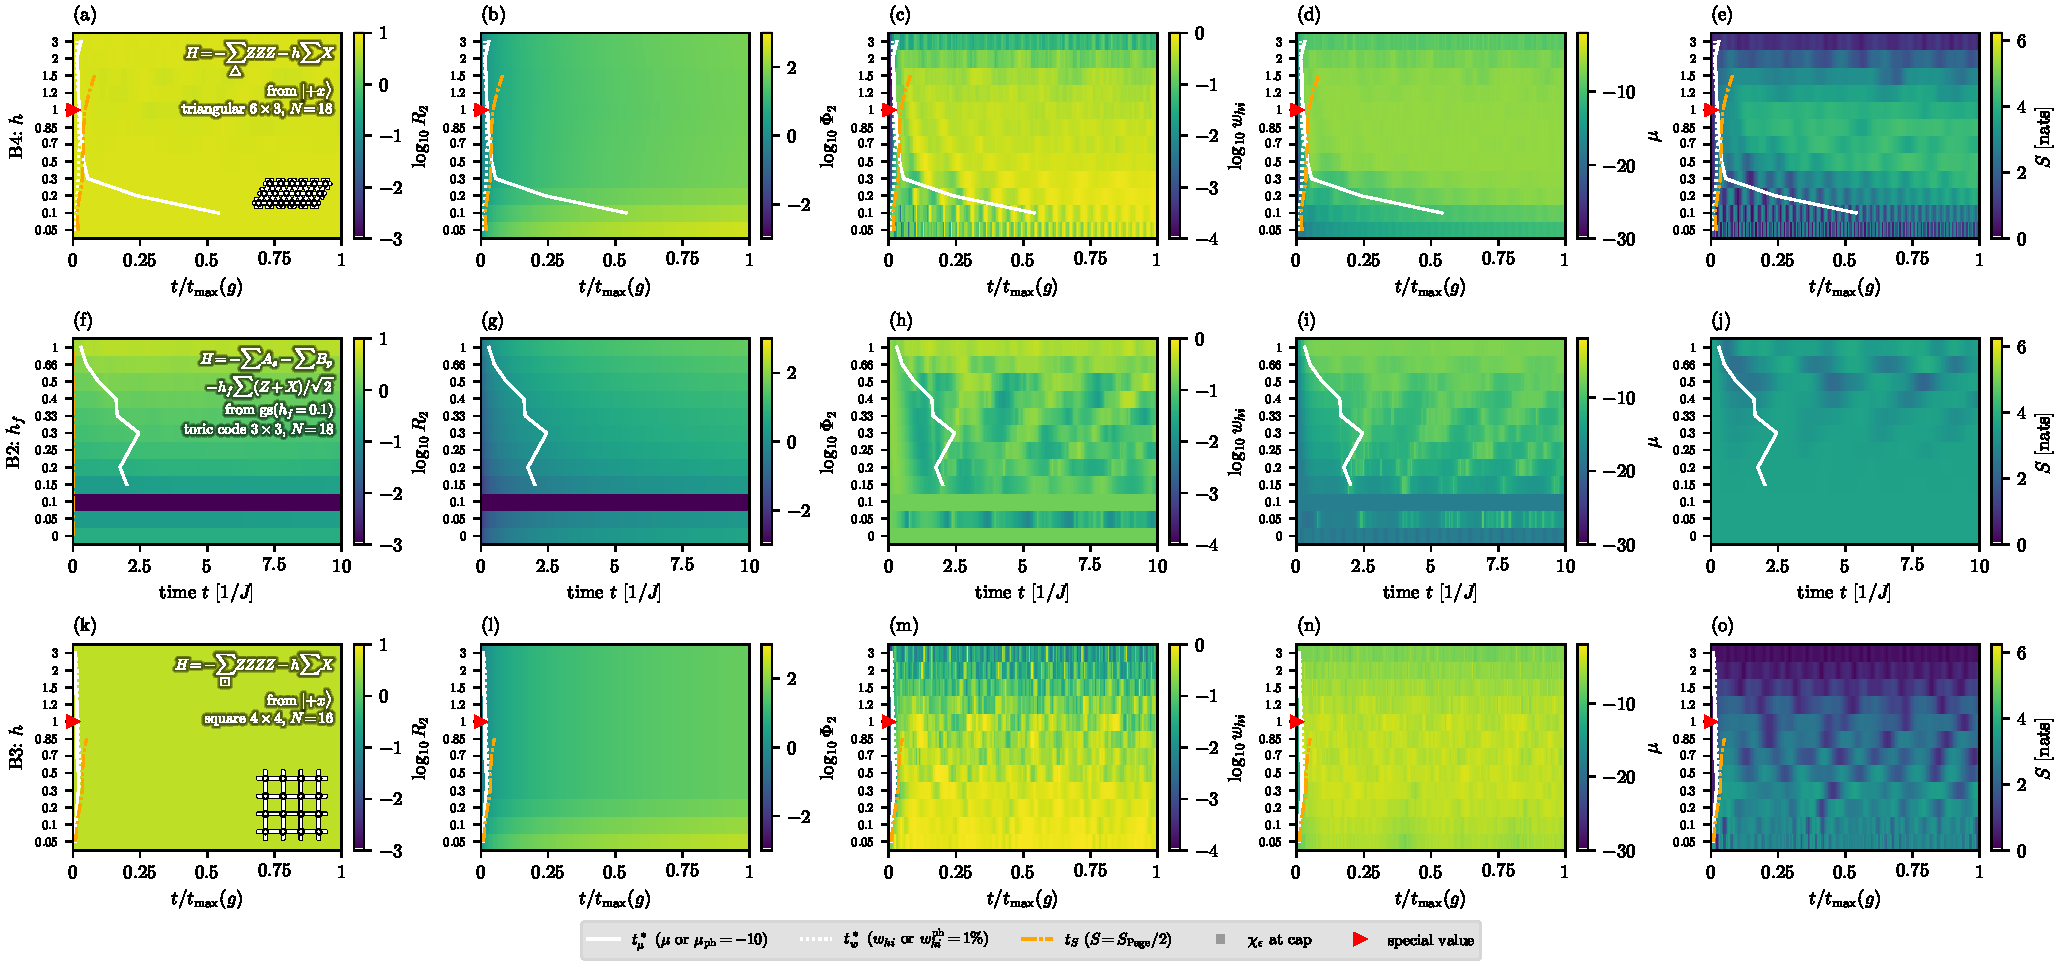
\includegraphics[width=\linewidth]{b2b/main_hl_1.pdf}
  \caption{\textbf{Predictors of the three highlighted quenches over time $t$ (horizontal) and control parameter
    (vertical, one row per grid point).} Rows of panels: (a)--(e) \BW{} from $\ket{+x}$, 18 spins, time in units of the run
    length $t_{\max}(h)=\min(300,\max(10,3/h))$; (f)--(j) \TC{} from the ground state at $h_f=0.1$, 18 spins;
    (k)--(o) \XM{} from $\ket{+x}$, 16 spins, time in units of $t_{\max}(h)$. Columns: few-body error rate $\log_{10}R_2$,
    its integral $\log_{10}\Phi_2$, high-order weight $\log_{10}\whi$, cumulant level $\mu$ (floor $-30$ = exactly
    two-body), entanglement entropy $S$ in nats (grey squares: times at which an MPS with discarded weight $10^{-3}$
    needs the largest possible bond dimension at the cut with the largest $S$).
    Lines on every panel: solid white, $\tmu$ ($\mu$ or $\mu_{\mathrm{ph}}$ first above $-10$); dotted white,
    $\tw$ ($\whi$ or $\whi^{\mathrm{ph}}$ first above $1\%$); dash-dotted orange, $t_S$ (first $S\ge\Spage/2$:
    $2.52$ nats for 16 spins, $2.87$ for 18). A line at the left edge means an onset at $t=0$ (all $\tw$ and $t_S$ of the
    toric code); a missing line means no onset within the run. Red triangles: self-dual point $h=1$ (assumed for
    Baxter--Wu, see \cref{app:issues}). Insets: Hamiltonian, start state, lattice (sketch omitted for the toric
    code). The toric-code row at $h_f=0.1$ is the start state itself (no quench).}
  \label{fig:main}
\end{sidewaysfigure}

\section{Toric code in a diagonal field: the only non-classical $\mu$-window}
\label{sec:toric}
\emph{The \TC{} is the only family with $\eta\approx0.7$ in which $\mu$ predicts an easy RBM at MPS-hard times, and
its windows are the largest of the non-trivial quenches} (\cref{fig:main}f--j, \cref{fig:abstract}).

\paragraph{The window.} For $h_f=0.05$--$0.4$ (all quenches with $0<h_f\le0.4$; $h_f=0.1$ is no quench),
$\tmu=1.6$--$2.45$ at 18 spins and $0.45$--$2.35$ at 12 spins. The window is $16$--$24\%$ of the save times at 18 spins
and $5$--$23\%$ at 12 spins. For $h_f\ge0.5$ it shrinks to $3$--$7\%$. $\mu_{\mathrm{ph}}$ crosses first in most rows;
$\mu$ stays near $-15$ for $h_f\le0.15$ up to $t=10$. $R_2$ grows smoothly with $h_f$, from $0.2$ ($h_f=0.15$) to $3.7$
($h_f=1$) at late times, without a sharp change.

\paragraph{The quench to the pure toric code.} At $h_f=0$, $\mu$ and $\mu_{\mathrm{ph}}$ stay below $-10$ for the whole
run (window $100\%$). The final Hamiltonian is a sum of commuting stabilisers, much like the classical quench limits of
the two-spin families, so we do not count this point as evidence.

\paragraph{The entanglement is there from the start.} The state is MPS-hard at $t=0$: $S=3.59$ nats at 18 spins,
above the threshold $2.87$, and it barely changes during the run. We attribute this to the area-law entropy of the
topological ground state across a cut that crosses the torus twice; it is not generated by the quench. The window thus
measures how long the quench keeps the state simple, not how fast it becomes complex.

\paragraph{The high-order weight disagrees.} $\whi=0.13$ already at $t=0$, so $\tw=0$ for every $h_f$. The start
state is close to the toric-code ground state, which has an exact RBM with $\alpha=1$~\cite{DengPRB17}, and $\mu=-18$
at $t=0$. We read this as a failure of $\whi$ for this class of states, but did not test it.

\begin{finding}[: toric code in a diagonal field]
From the toric-code ground state, $\mu$ predicts an easy RBM for $16$--$24\%$ of the save times ($t\lesssim2.5$) for
$0<h_f\le0.4$ at 18 spins ($5$--$23\%$ at 12 spins), at $\eta=0.71$. The state is MPS-hard throughout because the start
state is already entangled. $\whi$ calls even the start state hard, although that state is close to one with an exact
RBM.
\end{finding}

\section{Weak-field three-spin quenches: $\mu$ says easy, $\whi$ says hard, $R_2$ is large}
\label{sec:threespin}
\emph{At weak fields the \BW{} and the \NM{} are predicted easy by $\mu$ long after the state first becomes
MPS-hard; $\whi$ calls them hard almost at once, and $R_2$ stays large} (\cref{fig:main}a--e, \cref{fig:abstract}).

\paragraph{The cumulant level.} In the Baxter--Wu quench, $\mu$ and $\mu_{\mathrm{ph}}$ stay below $-10$ until
$\tmu=3.6$ ($h=0.2$), $16.2$ ($h=0.1$) and beyond $t_{\max}=60$ ($h=0.05$). The state first becomes MPS-hard at
$t_S=0.4$--$1.2$, but at $h\le0.1$ its entropy oscillates and exceeds the threshold $2.87$ nats only intermittently
(largest $S$: $3.1$--$3.2$ nats; \cref{fig:main}e). The window is therefore $5\%$, $10\%$ and $19\%$ of the save times
(at $h=0.2$, $0.1$, $0.05$), and below $2\%$ for $h\ge0.3$. The Newman--Moore quench gives $31\%$, $10\%$, $3.5\%$,
$3.5\%$ and $1\%$ at $h=0.05$, $0.1$, $0.2$, $0.3$, $0.5$. The windows shrink steadily with $h$; there is no sharp
boundary.

\paragraph{The few-body error rate.} $R_2$ starts at $6$ for every $h$ and stays between $4.9$ and $6$ for the whole
run (\cref{fig:main}a). The value is analytic: from $\ket{+x}$ the velocity $v(s,0)$ contains the classical energy
$\sum_\triangle s_is_js_k$, whose 36 triangle terms are orthogonal to all one- and two-body functions under the
uniform weight, so $R_2(0)=\sqrt{36}$. Since $R_2$ is large for every $h$, it does not separate the weak-field quenches
from the others. $R_4$, which admits three- and four-spin clusters, is $0$ at $t=0$ and stays below $0.35$ for
$h\le0.1$ (\cref{fig:appx}).

\paragraph{The high-order weight.} $\whi$ crosses $1\%$ at $\tw=0.15$--$0.3$ for every $h$ (at $h\le0.1$ this is
the first or second save time, so an upper bound), and reaches $43\%$ at $t=30$ for $h=0.05$, while $\mu\approx-12$.
We attribute the difference to what the two measure: at weak field the log-amplitude presumably varies only by
$O(h)$, so a small absolute high-order part is already a large relative weight.

\paragraph{Why this matters.} The phase of this state is close to $e^{it\sum_\triangle s_is_js_k}$, an exactly
three-body function. An RBM with weights of order one can write three-body phases, but a TDVP run started from a
product state with zero hidden biases does not move in the direction of odd three-body terms (previous report). So
$\mu$ asks whether the state is \emph{representable}, $R_2$ whether a two-body \emph{motion} can follow it. We interpret
the disagreement as this difference, but did not test it.

\begin{finding}[: three-spin quenches]
In the Baxter--Wu and Newman--Moore quenches at $h\le0.1$, $\mu$ predicts an easy RBM for $10$--$31\%$ of the save
times while the state is MPS-hard. $\whi$ exceeds $1\%$ by $t=0.3$, and $R_2$ stays between $4.9$ and $6$
(Baxter--Wu). Only RBM runs can tell which predictor is right.
\end{finding}

\section{Hard everywhere: plaquette and mixed models}
\label{sec:negative}
\emph{From $\ket{+x}$, the \XM{} and the two mixed families are hard by every predictor within $t\le0.6$, at every
value of the control parameter} (\cref{fig:main}k--o, \cref{app:full}).
\begin{itemize}
  \item \XM{}: $\tmu\le0.6$ and $\tw\le0.6$; no window at any $h$. $R_2$ is constant in time and equals the energy
    spread, $R_2=\Delta E=4$ from $\ket{+x}$: the subsystem symmetries (spin flips of a whole row or column) forbid every
    two-body cluster, so only the constant part of $v$ can be fitted.
  \item Ising plus plaquette (B6) and Baxter--Wu plus Ising (B7): $\tmu,\tw\le0.5$, and $S$ reaches $4.5$--$5.0$
    nats. The added two-spin term, meant to build up RBM weights, does not open a window for any $K$ or $\lambda$.
  \item Ground-state starts at $h=1.5$ (\cref{fig:full2,fig:full3}): Xu--Moore and Baxter--Wu have $\mu>-10$ already
    at $t=0$. Newman--Moore opens $\mu$-windows of $9\%$ and $1.5\%$ at $h=0.1$, $0.3$ only. The quenches to the
    classical point $h=0$ give $\whi$-windows of about $60\%$ in Xu--Moore and Newman--Moore, which we do not count
    (diagonal final Hamiltonian).
\end{itemize}

\section{Verdict}
\label{sec:verdict}
\paragraph{Answers.}
\begin{itemize}
  \item \emph{Are there multi-spin families with a predicted easy/hard split along the control parameter?}
    According to $\mu$, there are families whose window shrinks with the control parameter: the toric code in a
    diagonal field ($16$--$24\%$ for $0<h_f\le0.4$, $3$--$7\%$ above) and the Baxter--Wu and Newman--Moore quenches (from
    $19$--$31\%$ at $h=0.05$ to below $5\%$ for $h\ge0.2$). None has a sharp boundary. According to $\whi$, the
    $\ket{+x}$ and toric-code quenches have no window (largest $0.5\%$). $R_2$ has no threshold yet, but stays large
    in the three-spin quenches.
  \item \emph{Is any predicted window also non-classical?} Only the toric code ($\eta=0.71$), and there the MPS-hardness
    comes from the start state.
  \item \emph{How far can $\mu$ be trusted?} On the two reference quenches with RBM data, $\mu$ tracks the $\alpha=1$
    infidelity as well as or better than $R_2$ and $\whi$ (Spearman $0.93$ against $0.51$ and $0.47$ in the Rydberg Ising
    quench, all $0.91$ in the transverse-field Ising quench). Its onset was $1.1$--$2.6$ times late in the Rydberg
    quench but early at large fields in the transverse-field Ising quench (\cref{app:validation}). If the multi-spin
    quenches behave like the Rydberg quench, the $\mu$-windows above are upper bounds; this is untested.
\end{itemize}

\paragraph{Recommended RBM runs.}
The predictors disagree most clearly on three sets of points: the toric code at $h_f=0.15$, $0.3$ (12 spins first,
then 18) and the Newman--Moore quench at $h=0.05$, $0.1$, $0.2$ (16 spins), both cheap with TDVP on exact sums over all
configurations; and the Baxter--Wu quench at $h=0.05$, $0.1$ (18 spins) only if that size is affordable. The three-spin
quenches need non-zero initial hidden biases, otherwise the RBM does not move (previous report).

\paragraph{Limitations.}
\begin{itemize}
  \item No RBM was run; every statement about RBMs is a prediction.
  \item The thresholds $\mu=-10$ and $\whi=1\%$ were calibrated on two-spin quenches. Their meaning for three- and
    four-spin states is untested, and the two disagree here.
  \item 12--18 spins. The MPS-hard threshold is half the random-state entropy at that size, $e^S\approx6$--$18$; this
    is small in absolute terms.
  \item The toric code in a $Z$ field (B1) and the ground-state start of Baxter--Wu give no usable prediction
    (\cref{app:issues}).
\end{itemize}

\FloatBarrier
\appendix

\section{Notation}
\begin{center}
\begin{tabular}{lll}
  \toprule
  symbol & name & defined in \\
  \midrule
  $s$, $s_A$ & spin configuration, cluster function & \cref{sec:defs} \\
  $v(s)$ & local velocity $-i(H\psi)/\psi$ & \cref{sec:defs} \\
  $R_k$, $\Phi_k$ & few-body error rate, accumulated error & \cref{sec:defs} \\
  $c_A$, $\mu$, $\mu_{\mathrm{ph}}$ & cluster coefficients, cumulant levels & \cref{sec:defs} \\
  $\whi$, $\whi^{\mathrm{ph}}$ & high-order cluster weights & \cref{sec:defs} \\
  $S$, $\Spage$ & half-cut entropy, random-state value & \cref{sec:defs} \\
  $\tmu$, $\tw$, $t_S$ & onset times & \cref{sec:defs} \\
  $\eta$ & non-classicality & \cref{sec:defs} \\
  $\chi_\epsilon$ & MPS bond dimension for discarded weight $10^{-3}$ & \cref{fig:appx} \\
  $g$; $h$, $h_f$, $K$, $\lambda$ & control parameter; its value per family & \cref{tab:families} \\
  $A_s$, $B_p$ & toric-code star and plaquette & \cref{sec:setup} \\
  $t_{\max}$ & run length & \cref{sec:setup} \\
  $I$ & RBM infidelity $1-\lvert\braket{\psi_{\mathrm{ED}}|\psi_{\mathrm{RBM}}}\rvert^2$ & \cref{app:validation} \\
  \bottomrule
\end{tabular}
\end{center}

\section{All families}
\label{app:lattices}
\begin{table}[h]
\centering\small
\resizebox{\linewidth}{!}{%
\begin{tabular}{llllll}
  \toprule
  ID & Hamiltonian & lattice ($N$) & start & control $g$ & $\eta$ \\
  \midrule
  B1 & toric code $-h_f\sum Z$ & toric $2\times3$ (12), $3\times3$ (18) & gs($h_f=0.1$) & $h_f\in[0,1]$ & 0.50--0.71 \\
  B2 & toric code $-h_f\sum(Z+X)/\sqrt2$ & toric $2\times3$, $3\times3$ & gs($h_f=0.1$) & $h_f\in[0,1]$ & 0.71 \\
  B3 & $-\sum_\square ZZZZ-h\sum X$ & square $4\times4$ (16) & $\ket{+x}$; gs($h=1.5$) & $h$ & 0.00--0.95 \\
  B4 & $-\sum_\triangle ZZZ-h\sum X$ & triangular $6\times3$ (18) & $\ket{+x}$; gs($h=1.5$) & $h$ & 0.00--0.91 \\
  B5 & $-\sum_{\triangle_\uparrow} ZZZ-h\sum X$ & triangular $4\times4$ (16) & $\ket{+x}$; gs($h=1.5$) & $h$ & 0.00--0.95 \\
  B6 & $-\sum ZZ-K\sum_\square ZZZZ-0.5\sum X$ & square $4\times4$ & $\ket{+x}$ & $K\in[0,2]$ & 0.20--0.33 \\
  B7 & $-\sum_\triangle ZZZ-\lambda\sum ZZ-0.5\sum X$ & triangular $4\times4$ & $\ket{+x}$ & $\lambda\in[0,2]$ & 0.13--0.33 \\
  \midrule
  G4 & $-\sum r^{-6}ZZ-h_f\sum X$ & square $4\times3$ (12) & gs($h_f=4$) & $h_f$ & 0.00--0.98 \\
  R1 & Rydberg, $(\Omega/2)\sum X+\sum V_{ij}n_in_j$ & square $4\times3$ & $\ket{+x}$ & $\Omega/V_{nn}$ & 0.00--0.45 \\
  S1 & toric code $+\epsilon\sum Z$ & toric $2\times3$ & tilted, $\theta=\pi/4$ & $\epsilon$ & 0.63--0.71 \\
  I5 & $\sum_\triangle ZZZ+h_x\sum X$ & triangular $4\times3$ & $\ket{+x}$ & $h_x$ & 0.00--0.33 \\
  \bottomrule
\end{tabular}}
\caption{Families of the screen (above the line) and two-spin and earlier multi-spin reference families recomputed with
  the new predictors (below). Sums run over nearest-neighbour bonds ($ZZ$), all triangles ($\triangle$), up-triangles
  ($\triangle_\uparrow$), square plaquettes ($\square$). gs: ground state of the same Hamiltonian at the given parameter.
  $\eta$: range over the grid. Grids: 12 points per family (B), 8--13 (references); full lists in
  \texttt{rydberg\_screen.py}.}
\label{tab:families}
\end{table}

\paragraph{Lattices.} Periodic in both directions. Square and triangular tori are labelled by columns $x$ and rows $y$,
site $i=xL_y+y$; the entanglement cut separates the first $L_x/2$ columns from the rest. Triangular lattice vectors
$(1,0)$ and $(\frac12,\frac{\sqrt3}2)$; up-triangles $(x,y),(x+1,y),(x,y+1)$, down-triangles
$(x+1,y),(x,y+1),(x+1,y+1)$. Toric-code tori have one spin per link, ordered column by column (vertical links at $x$,
then horizontal links at $x+\tfrac12$); the cut runs between link midpoints $x\le1$ and $x>1$ on the $3\times3$ torus and
$x\le\frac12$ on the $2\times3$ torus.

\FloatBarrier
\section{Full matrices}
\label{app:full}
\Cref{fig:full1,fig:full2,fig:full3,fig:full4} show the main predictors for all 16 rows (families and starts),
\cref{fig:appx} the appendix predictors for the highlights. The full appendix matrices are in
\texttt{rydberg/figs/b2b/appx\_1.pdf} to \texttt{appx\_4.pdf}.

\newcommand{\fullcaption}{Layout, lines and colour scales as in \cref{fig:main}. Rows whose run length depends on the
  control parameter are shown against $t/t_{\max}(g)$. Red triangles: special values (the dual-TFI critical field
  $0.33$ of B1, self-dual points, reductions to earlier families, experimental values of the references).}
\begin{figure}[p]
  \centering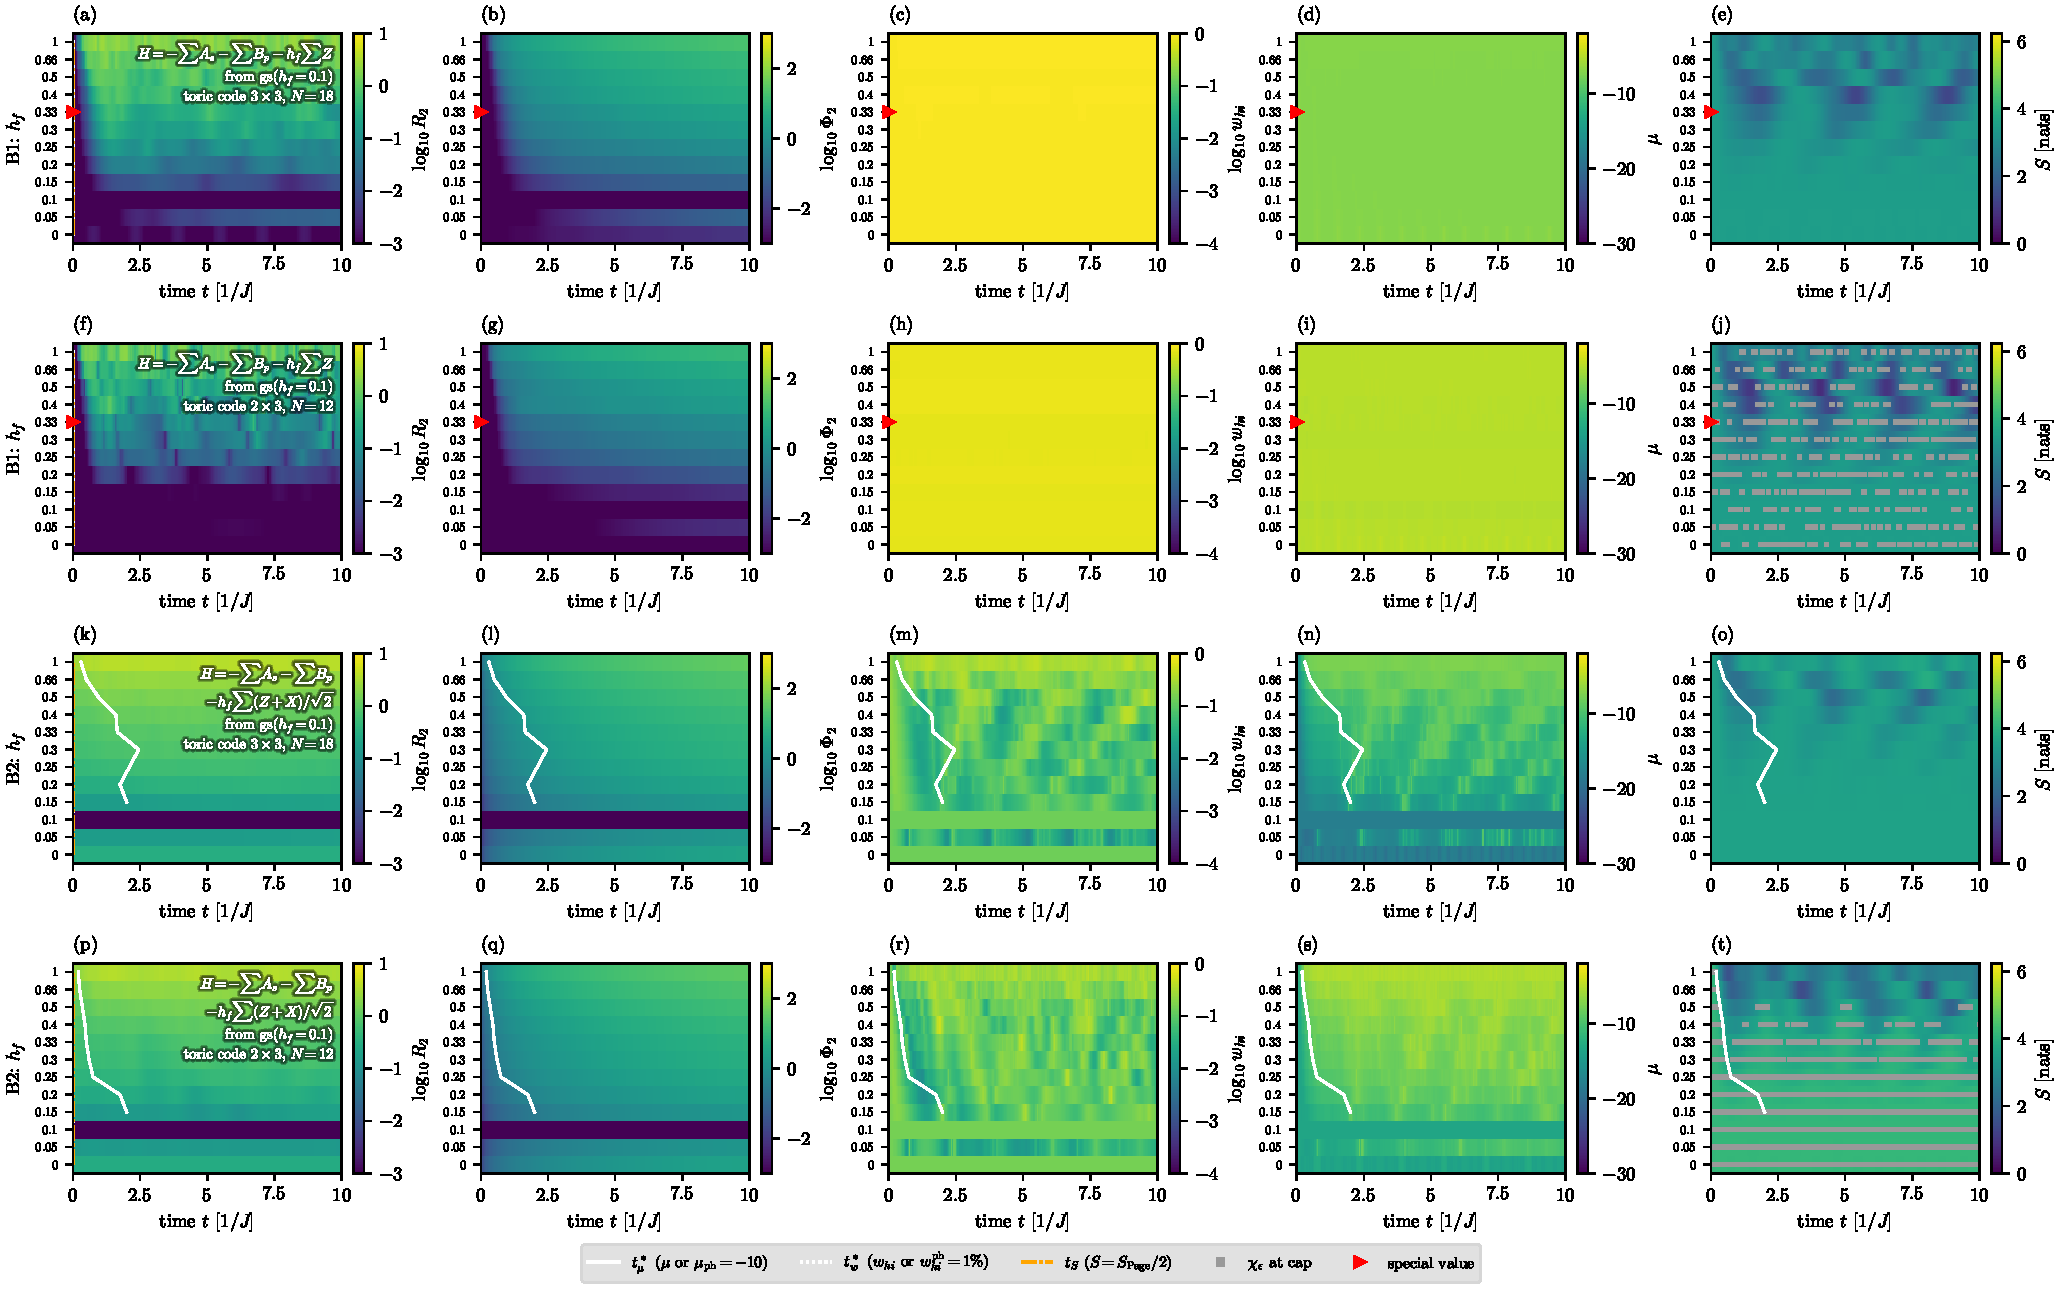
\includegraphics[width=\linewidth]{b2b/main_1.pdf}
  \caption{Toric code in a $Z$ field (B1) and in a diagonal field (B2), 18 and 12 spins. \fullcaption{} In B1 the
    state is confined to 256 (32) of $2^{18}$ ($2^{12}$) configurations and all cluster predictors are meaningless
    (\cref{app:issues}).}
  \label{fig:full1}
\end{figure}
\begin{figure}[p]
  \centering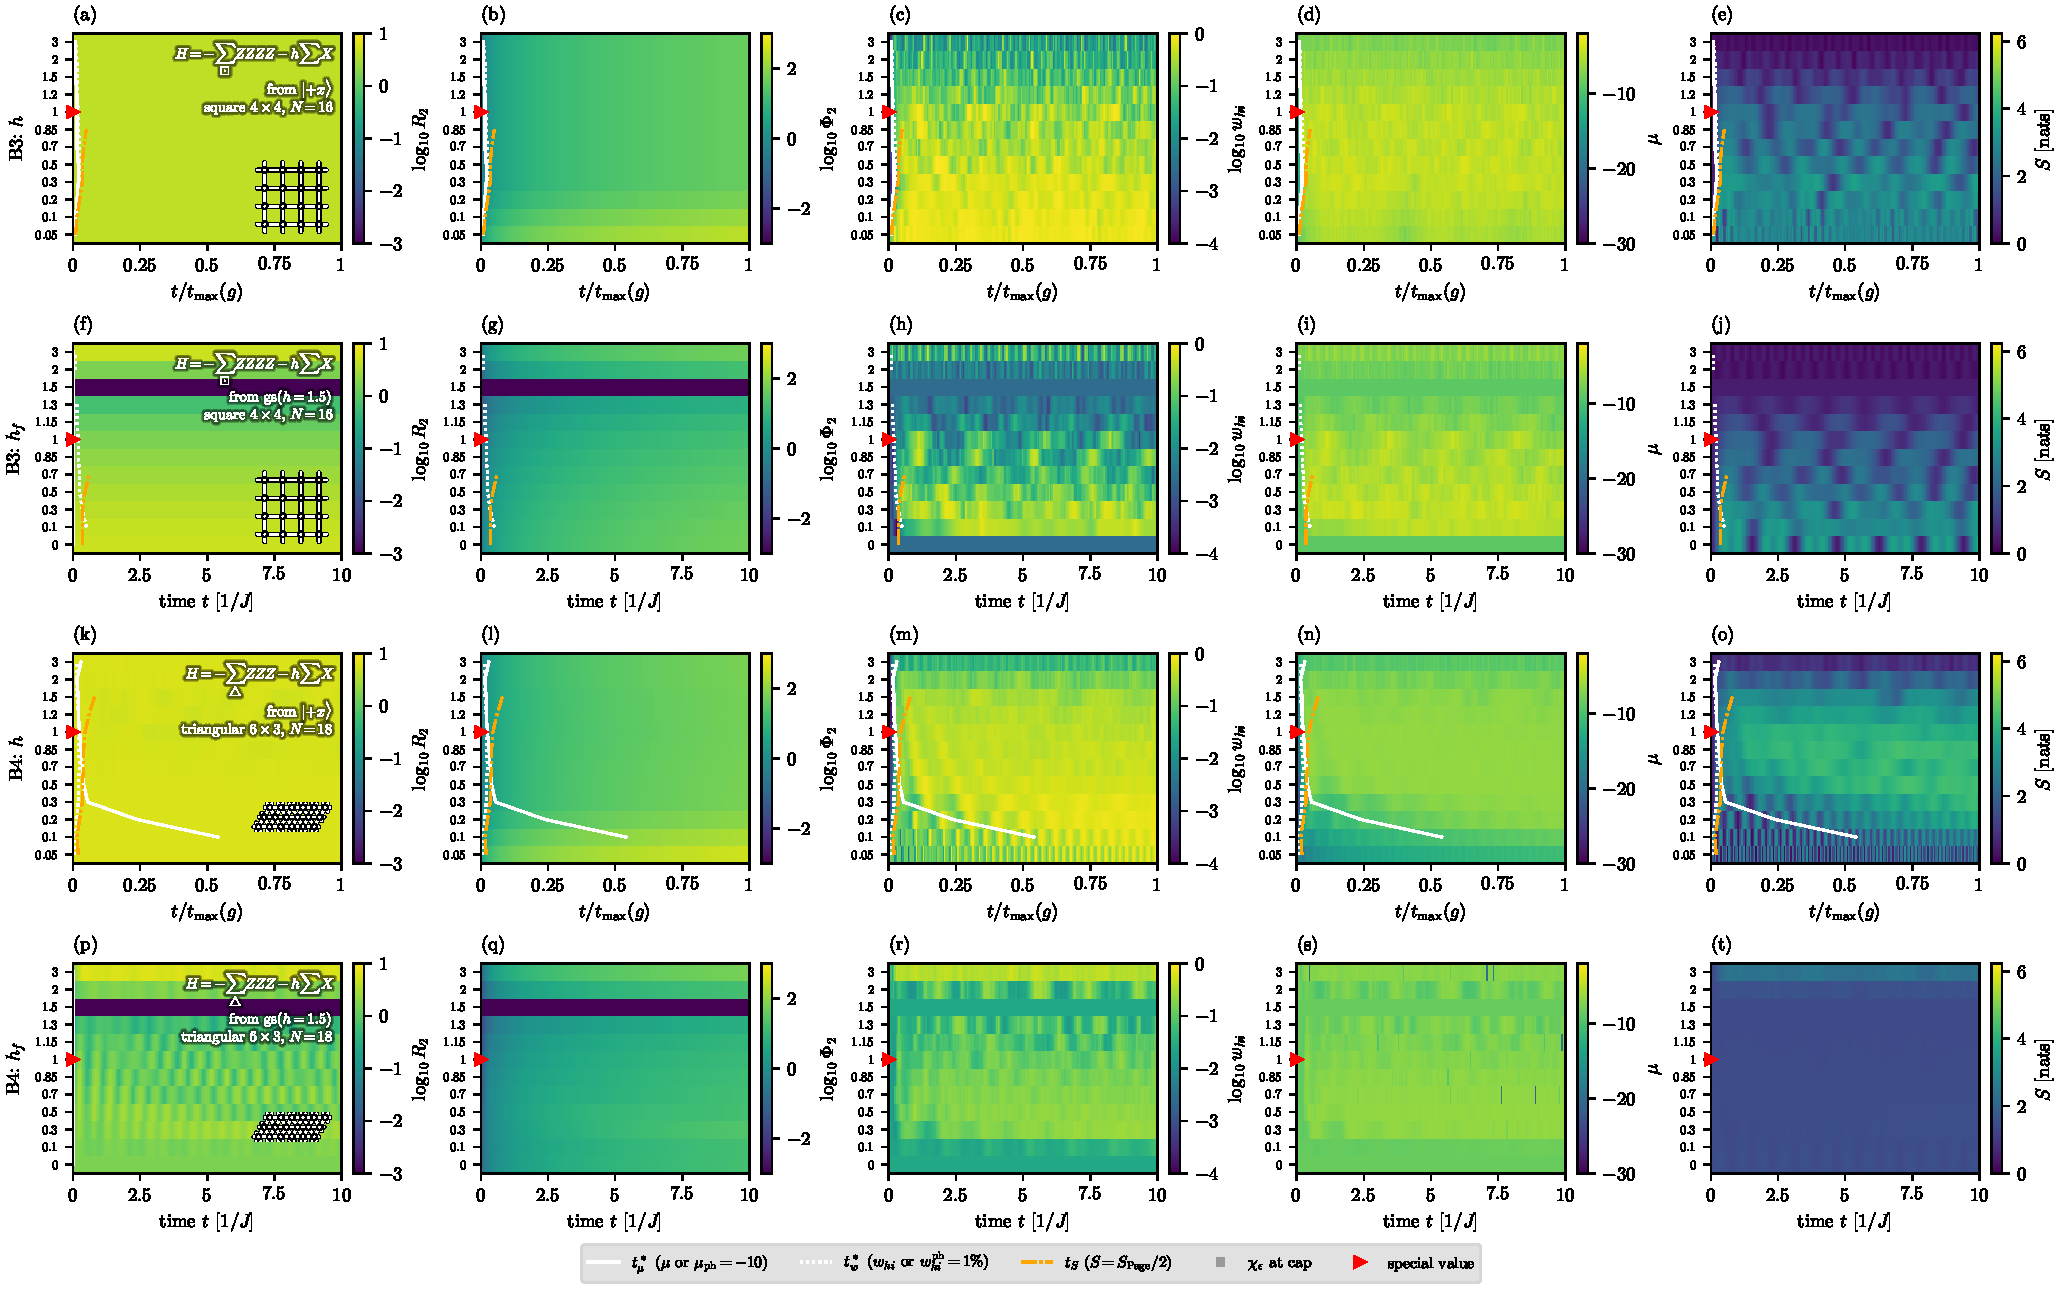
\includegraphics[width=\linewidth]{b2b/main_2.pdf}
  \caption{Xu--Moore (B3) and Baxter--Wu (B4), each from $\ket{+x}$ and from the ground state at $h=1.5$. \fullcaption{}
    The Baxter--Wu ground-state start is an ordered cat state (\cref{app:issues}).}
  \label{fig:full2}
\end{figure}
\begin{figure}[p]
  \centering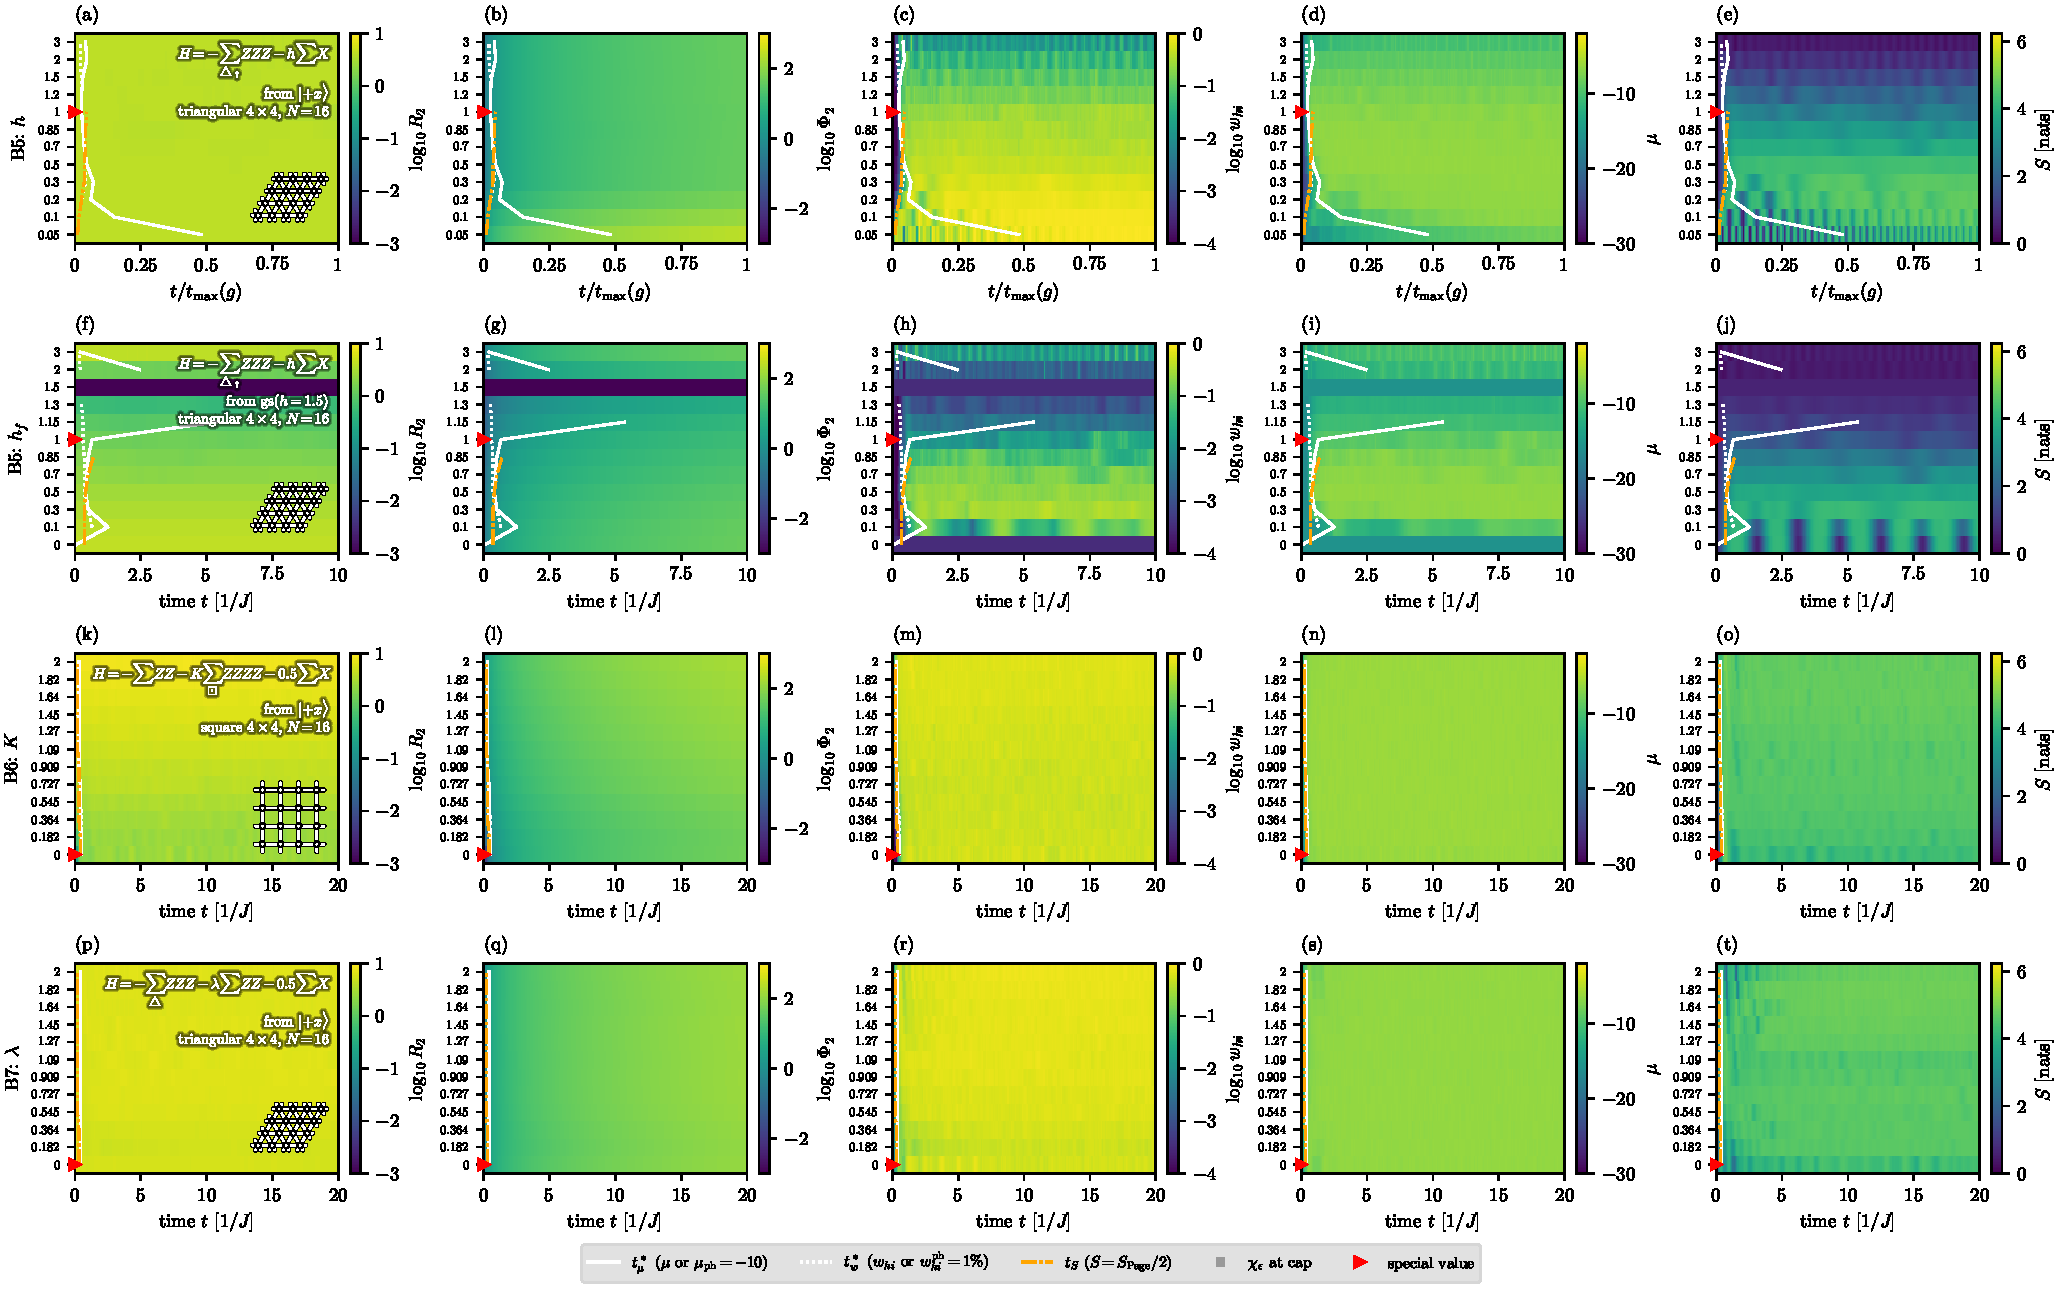
\includegraphics[width=\linewidth]{b2b/main_3.pdf}
  \caption{Newman--Moore (B5) from $\ket{+x}$ and from the ground state at $h=1.5$; Ising plus plaquette (B6) and
    Baxter--Wu plus Ising (B7) from $\ket{+x}$. \fullcaption{}}
  \label{fig:full3}
\end{figure}
\begin{figure}[p]
  \centering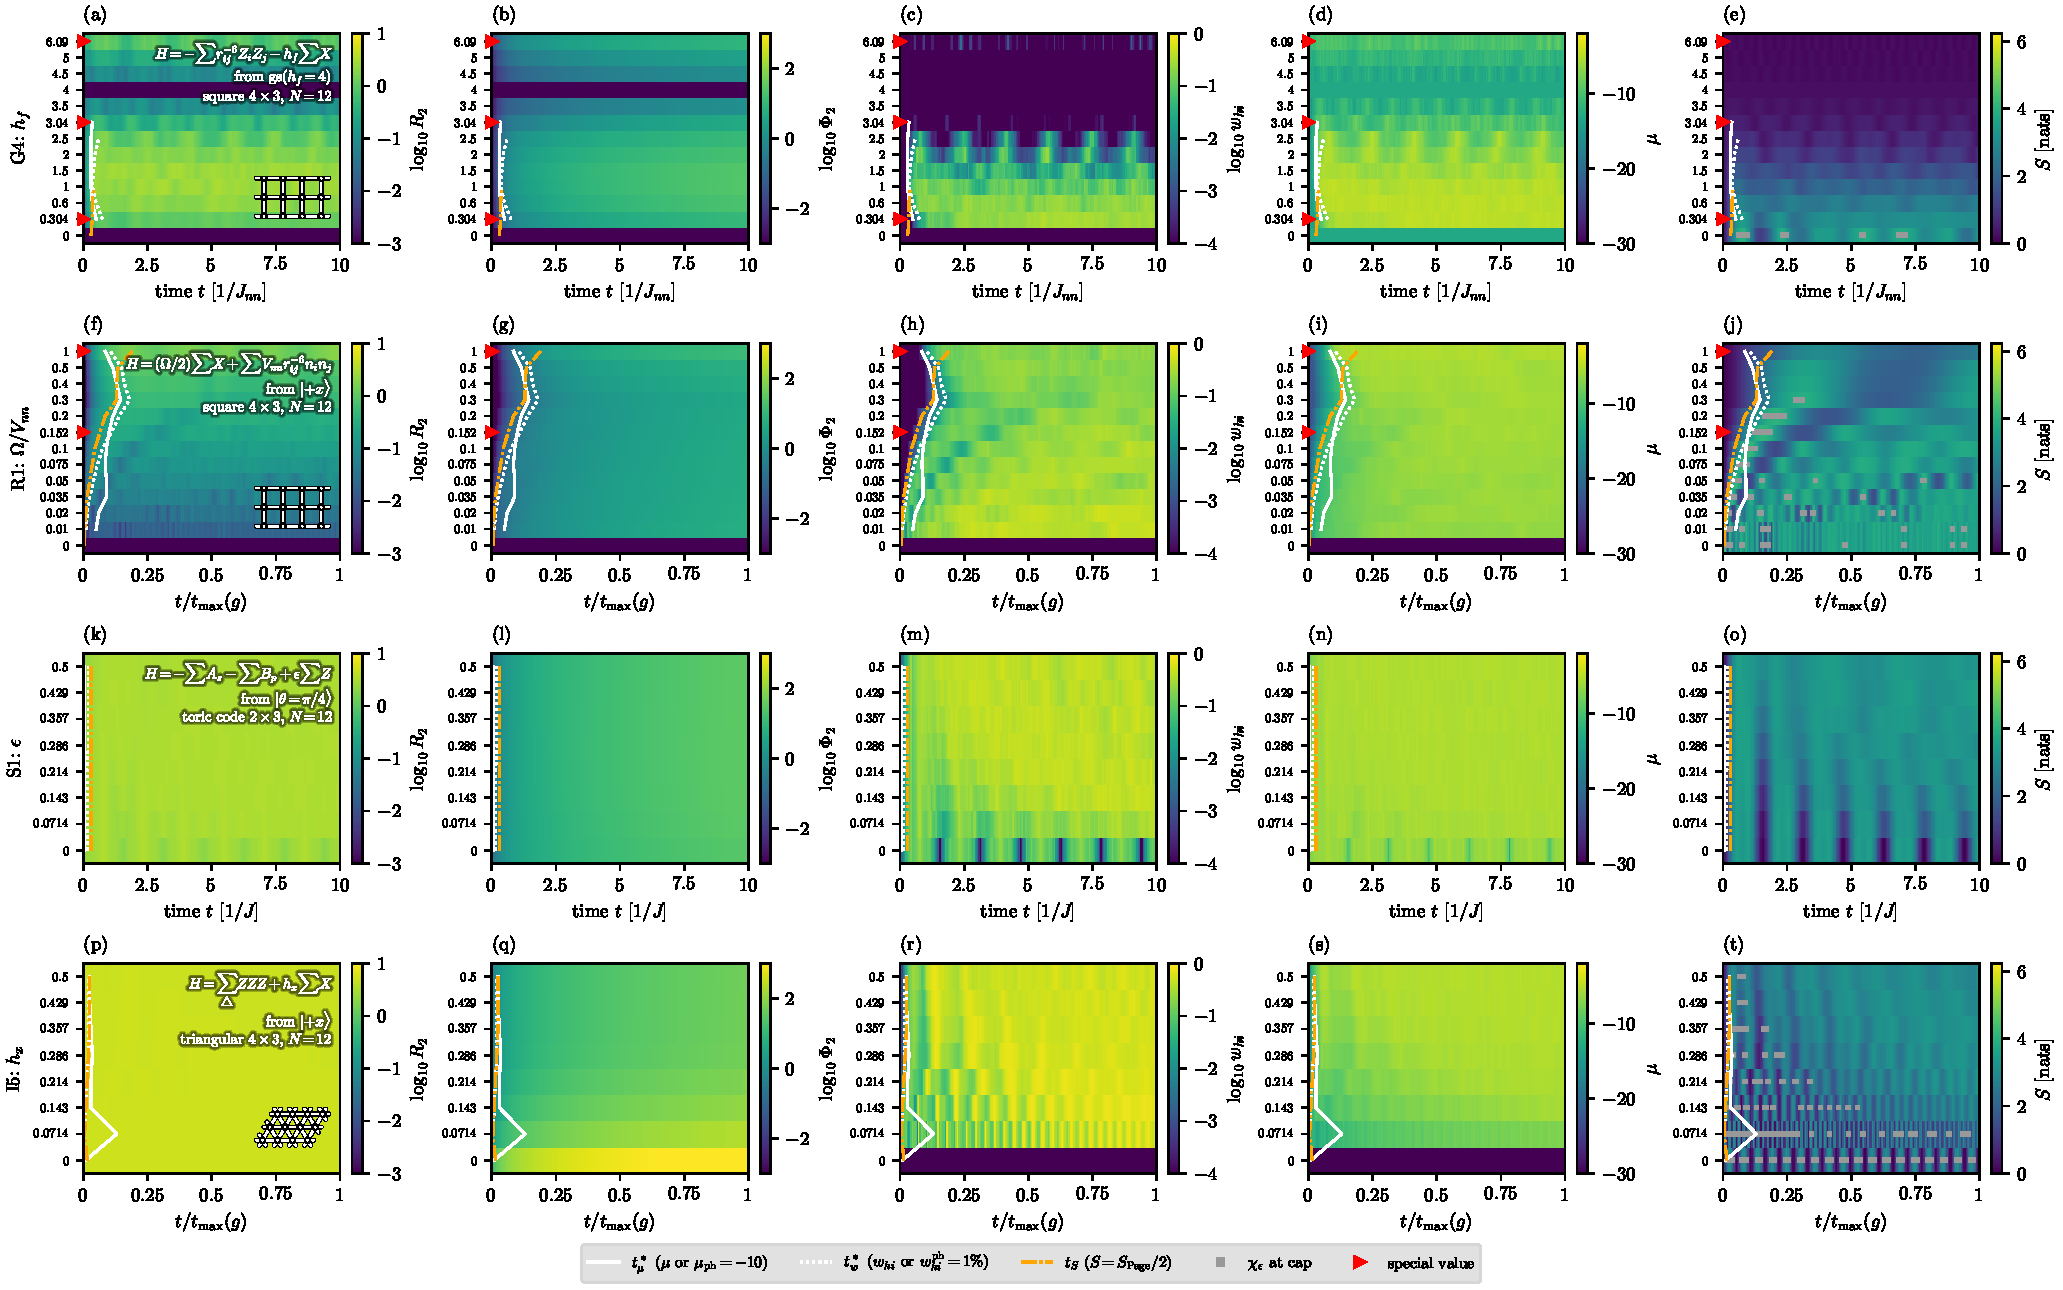
\includegraphics[width=\linewidth]{b2b/main_4.pdf}
  \caption{Reference families: 2D transverse-field Ising quench from its paramagnetic ground state (G4), Rydberg Ising
    quench (R1), toric code with a $Z$ field from a tilted product state (S1), three-spin Ising model in a field (I5),
    all 12 spins. \fullcaption{}}
  \label{fig:full4}
\end{figure}
\begin{figure}[p]
  \centering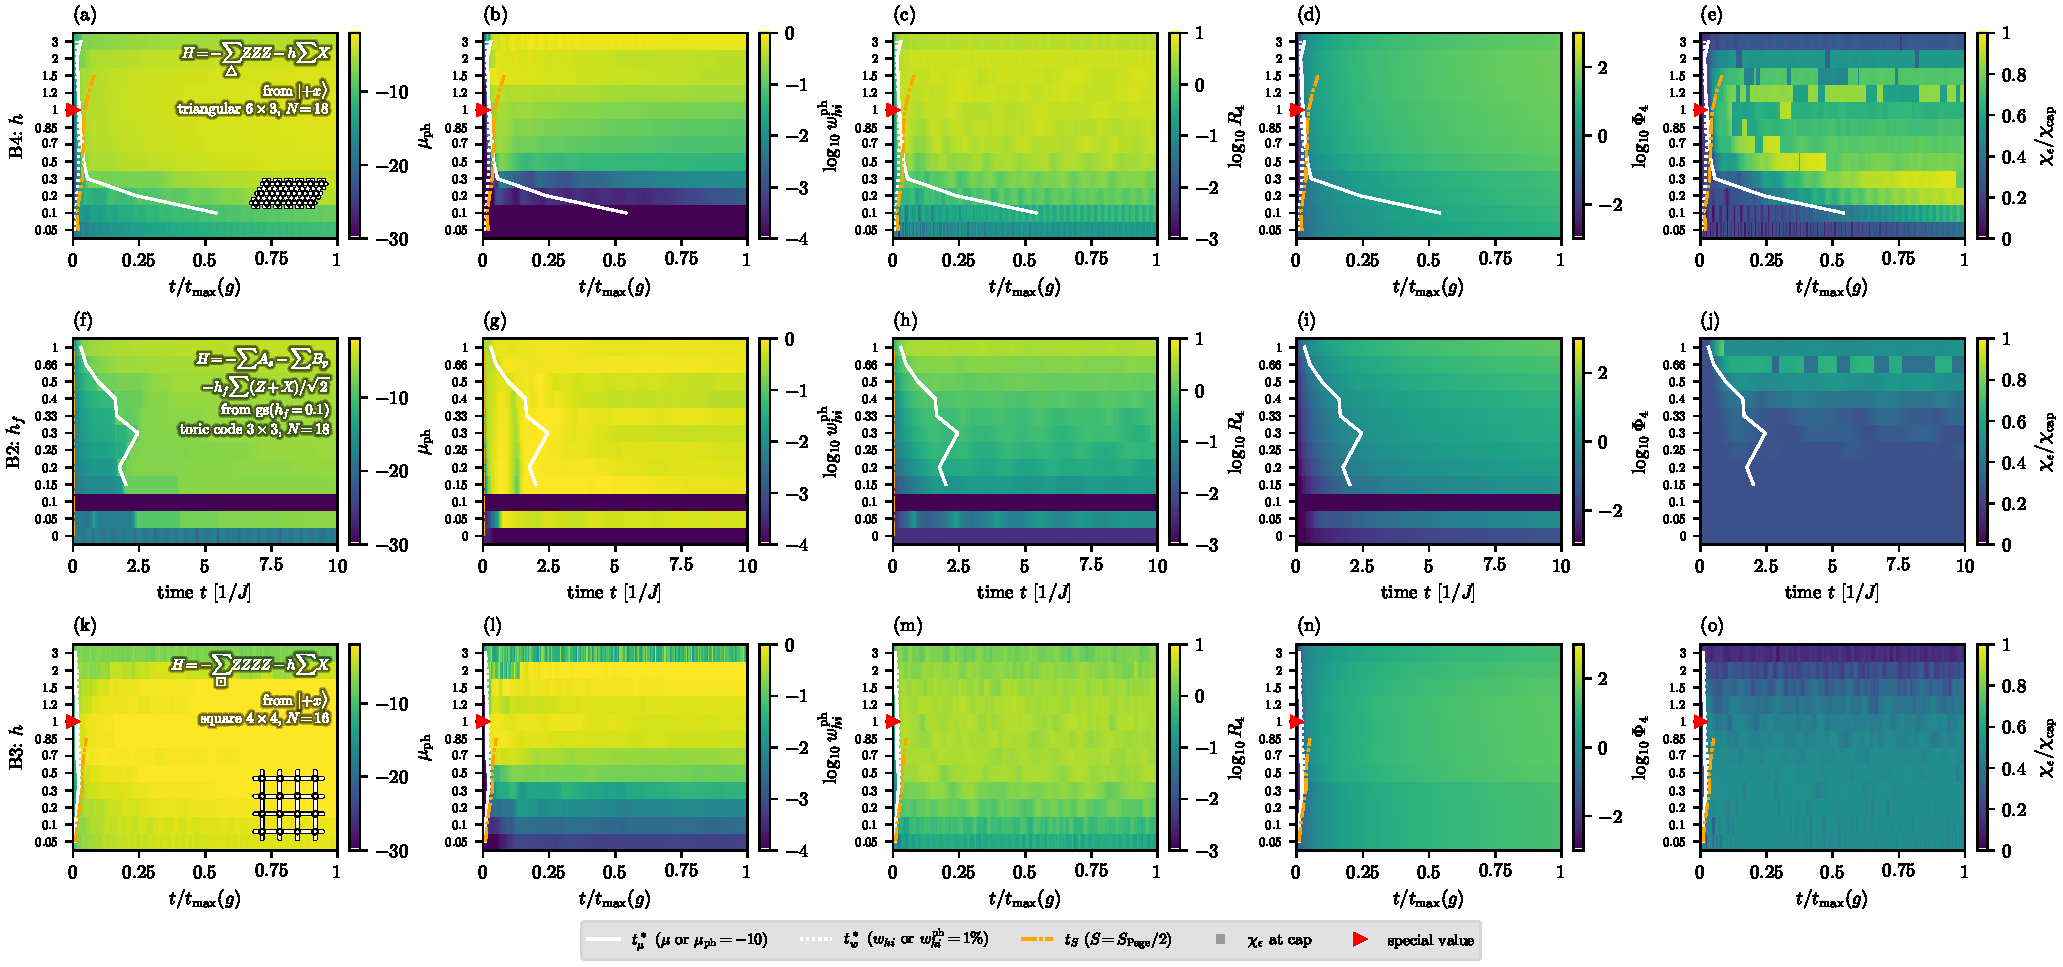
\includegraphics[width=\linewidth]{b2b/appx_hl_1.pdf}
  \caption{Appendix predictors of the three highlighted quenches (rows as in \cref{fig:main}). Columns: phase cumulant
    level $\mu_{\mathrm{ph}}$, phase high-order weight $\log_{10}\whi^{\mathrm{ph}}$, four-body error rate $\log_{10}R_4$,
    its integral $\log_{10}\Phi_4$, and the MPS bond dimension $\chi_\epsilon$ (discarded weight $10^{-3}$ at the cut
    with the largest $S$) as a fraction of its cap, $0$ for a product state. Lines as in \cref{fig:main}.}
  \label{fig:appx}
\end{figure}

\FloatBarrier
\section{Few-body error rate: implementation and checks}
\label{app:rk}
\paragraph{Normal equations in Walsh space.} With $s_As_B=s_{A\oplus B}$, the Gram matrix of the fit is
$G_{AB}=\sum_sp(s)s_{A\oplus B}$, one Walsh--Hadamard transform of $p$, and the right side is the transform of
$-i\,\overline{\psi}\,H\psi$ at the clusters $A$. No $2^N\times n_k$ matrix is formed ($n_2=172$, $n_4=4048$
unknowns at 18 spins). $G$ is real, so the real and imaginary parts are solved with one factorisation (least squares
with pivoted QR, relative cut-off $10^{-12}$, since $G$ is singular when $p$ has zeros). The residual is evaluated
directly, $\lvert\psi\rvert(v-f_c)=-i(H\psi)e^{-i\arg\psi}-\lvert\psi\rvert f_c$, not as a difference of two large
numbers.

\paragraph{Checks} (asserts in \texttt{rydberg2d.py}).
\begin{itemize}
  \item $R_2<10^{-10}$ at all times for a diagonal two-body $H$ (Rydberg interactions without drive).
  \item $R_2(0)<10^{-8}$ for the field quench of the 2D transverse-field Ising model from a ground state: there
    $v(s,0)$ is the constant plus $(1-h_f/h_0)$ times the two-body classical energy. $R_1(0)>10^{-3}$ for the same state.
  \item $R_2$ equals a dense least-squares fit on the explicit basis at 8 spins (random state, random $H$ with a
    three-spin term).
  \item Xu--Moore field quench from a ground state: $R_2(0)>10^{-2}$, $R_4(0)<10^{-7}$.
\end{itemize}

\paragraph{Analytic values seen in the data.} From $\ket{+x}$ the velocity at $t=0$ is $i$ times the classical
energy (plus a constant), so $R_2(0)$ is the root of the summed squared couplings of all terms with more than two spins:
$6$ (Baxter--Wu, 36 triangles), $4$ (Newman--Moore, 16 up-triangles; Xu--Moore, 16 plaquettes), $\sqrt{32}=5.66$ (B7),
$4K$ (B6). $R_4(0)=0$ for every product start and for the ground-state starts whose quench changes only the
$X$ field, since all terms have at most four spins; in the toric code in a diagonal field $R_4(0)=0.002$--$0.03$. In Xu--Moore $R_2(t)=\Delta E$ at all times (\cref{sec:negative}).

\section{Check against existing RBM data}
\label{app:validation}
\emph{On the two reference quenches with $\alpha=1$ RBM runs, $\mu$ predicts the infidelity as well as or better than the others; $R_2$ is
as good as $\mu$ in the transverse-field Ising quench and much worse in the Rydberg quench} (\cref{tab:rho}).

\begin{table}[h]
\centering\small
\begin{tabular}{lcccc}
  \toprule
  quench & $R_2$ & $\Phi_2$ & $\max(\whi,\whi^{\mathrm{ph}})$ & $\max(\mu,\mu_{\mathrm{ph}})$ \\
  \midrule
  2D transverse-field Ising (G4, 1941 points) & 0.91 & 0.88 & 0.91 & 0.91 \\
  Rydberg Ising (R1, 2170 points) & 0.51 & 0.83 & 0.47 & 0.93 \\
  \bottomrule
\end{tabular}
\caption{Spearman correlation between each predictor and $\log_{10}I$ of the $\alpha=1$ RBM ($I$: infidelity with the
  exact state), over all grid points and save times $t>0$; 12 spins, $4\times3$ cylinder. RBM data from the previous
  report (\texttt{data/rbm\_long.csv}).}
\label{tab:rho}
\end{table}

\paragraph{Onset times.} In the transverse-field Ising quench, $\tmu$ is within $0.15$ of the RBM failure time
$t^*_{\mathrm{inf}}$ (first $I>10^{-3}$) for $h_f\le2.5$, and early at the critical and large fields
($\tmu=0.35$--$0.4$ against $t^*_{\mathrm{inf}}=2.95$--$3.75$). In the Rydberg quench $\tmu$ is late by a factor
$1.1$--$2.6$ for every $\Omega/V_{nn}>0$ (e.g.\ $2.7$ against $1.65$ at $0.1$), while $\tw$ is early for
$\Omega/V_{nn}\le0.05$ ($2.1$--$3.0$ against $2.7$--$13.5$) and late above. Two further reference families of the previous report (dipolar XXZ and long-range Ising) were not
recomputed with $R_2$, and the three-spin family I5 changed Hamiltonian (\cref{app:deviations}), so the check covers two families.

\section{Problem cases}
\label{app:issues}
\paragraph{Toric code in a $Z$ field (B1).} The $Z$ field commutes with every plaquette $B_p$ and with the
non-contractible $Z$ loops, so the state stays in a sector of $2^{N}/2^{L_xL_y+1}$ configurations: 32 at 12 spins, 256
at 18. The amplitude is exactly zero elsewhere, so $\log\lvert\psi\rvert$ is dominated by the support indicator and
$\mu$, $\whi$ are above threshold at $t=0$. The fit for $R_4$ has rank equal to the support size and is exact for any
$v$ ($R_4\approx10^{-11}$), and $R_2$ has rank $127$ of the $256$ configurations. The model is dual to the 2D
transverse-field Ising model~\cite{Wegner71}; a fair test would use the dual variables, which this screen does not do.

\paragraph{Ground-state start of Baxter--Wu (B4).} The ground state at $h=1.5$ on the $6\times3$ torus has a gap of
only $3.8\times10^{-4}$ and $S(0)=1.40\approx\ln4$: this looks like a cat state of the four ordered Baxter--Wu
ground states, not the paramagnet intended by the plan. Possible causes, not tested: the transition lies above $h=1.5$
at this size; the model is not self-dual at $h=1$ as assumed; or the start state was prepared incorrectly. The gap stayed above the warning level $10^{-4}$, so no warning was
printed. This row is not interpreted.

\section{Numerical details}
\label{app:numerics}
\begin{itemize}
  \item 186 runs (144 new, 42 reference), 44 parallel processes, 2.5\,h wall time, 82 CPU hours. Per run: under 1\,min
    at 12 spins, 10--20\,min at 16, 53--138\,min at 18. The four-body fit dominates at 16 and 18 spins (about 7\,s per save
    time for full rank, 20\,s for the rank-deficient B1 fit).
  \item Peak memory: about 2.8\,GB per 18-spin run.
  \item Ground-state gaps of the pre-quench Hamiltonian: toric code $1.7\times10^{-3}$ (12 spins), $2.4\times10^{-3}$ (18,
    $Z$ field) and $1.5\times10^{-2}$, $1.2\times10^{-3}$ (diagonal field); Xu--Moore $2.4$; Newman--Moore $2.3$; Baxter--Wu
    $3.8\times10^{-4}$.
  \item Data in \texttt{rydberg/data/b2b/}: raw files per run, gathered files per family, the onset table
    \texttt{summary.csv} and the check tables \texttt{validate\_rho.csv}, \texttt{validate\_onsets.csv}.
  \item Scripts in \texttt{rydberg/}: \texttt{rydberg\_screen.py} (with the environment variable
    \texttt{SCREEN=data/b2b} and the command \texttt{run 4}), \texttt{b2b\_summary.py}, \texttt{b2b\_validate.py},
    and \texttt{rydberg\_figs.py} with the command \texttt{b2b}.
\end{itemize}

\section{Deviations from the plan}
\label{app:deviations}
The plan is \texttt{check\_time\_evolution/plans/plan\_beyond2body.md}.
\begin{itemize}
  \item \emph{Triangles fixed.} On a triangular torus with three rows, the old \texttt{triangles()} also returned the
    three-site loops that wind around the torus (28 instead of 24 on the $4\times3$ torus). It now returns the faces.
    The reference family I5 therefore has 4 fewer three-spin terms than in the previous report.
  \item \emph{Toric-code site order} changed to column by column, so the entanglement cut is spatial. The reference
    S1 has different $S$ than in the previous report.
  \item $\whi$ is set to $0$ for a flat amplitude (\cref{sec:defs}); onset times use the earlier of the amplitude
    and phase crossing.
  \item The support size and the rank of the fits were added to the output to detect cases like B1.
  \item No $R_2$ threshold line: the paper draft with the threshold was not available to check its size rescaling.
  \item The full matrices are split into four pages of four rows.
  \item The window is the fraction of save times that are MPS-hard and before the onset, not the time between $t_S$
    and the onset as in the plan, because $S$ oscillates around the threshold at weak fields.
  \item Highlights were chosen by the author of this report, not by the user.
\end{itemize}

\bibliographystyle{unsrt}
\bibliography{refs}
\end{document}
